\chapter{Introduction}
\thispagestyle{fancy} % this is magic. put it after every \chapter{...}
\section{Self Driving Cars}

The problem of traffic theory is generally to understand human behavior on the road and to use this knowledge for optimizing infrastructure. Determining when lanes should be added, where turns and bridges should be made, what the speed limit should be are all considerations that require engineers to turn to traffic theory. However, recent developments have raised new questions in traffic theory concerning a new kind of driver: the autonomous car. 

In theory, the efficiency of a highway system could be improved by the mere presence of these self-driving cars rather than the building of new lanes and roads. Jiang et al. \cite{jiang} cite various companies’ innovations including adaptive cruise control, lane change assistance, and vehicle-vehicle communication as game changers in traffic behavior.
Holland \cite{holland} found that small disturbances in traffic flow propagate down through lanes of cars causing traffic jams, a result also found by MIT \cite{mit}. A system of cooperating self-driving cars would likely be less prone to this kind of jam propagation. This is likely to be true because self driving cars can be programmed with optimal driving strategies that do not propagate disturbances backward. One aspect of these optimal strategies would be the avoidance of causing disturbances in the first place, something human drivers can do simply by changing lanes poorly.

\section{Kerner’s Three Phase Traffic Theory}
Kerner \cite{kerner} proposes that all traffic is divided into one of three states. The first state is called free flow, and it describes a state of traffic in which cars are separated far enough that drivers have no need to respond to the actions of cars around them. We assume that autonomous cars will have no effect on free flow traffic since this precludes the presence of any jam for cooperative thinking to optimize. 

We will instead focus on the effects of autonomous cars on the efficiency of highways in states of synchronized flow and wide moving jams which are the likely to be affected by collaborative thinking. Wide moving jams and synchronized flow are both states in which cars’ movements are determined by the cars surrounding them. Kerner distinguishes the two states by how their downstream fronts propagate. A wide moving jam propagates backward at a fixed velocity while the synchronized flow phase does not.

\section{Definitions}
We choose to measure the efficiency of a highway by its throughput. Throughput is defined as the number of cars that pass through a slice of a highway in a specific period of time. We will denote throughput by the letter “q” and use cars per second as its unit of measurement. Kerner refers to this measurement as flow and sometimes as volume, but also refers to the state of traffic (free flow, synchronized flow, wide moving jam) as kinds of flow. For the sake of clarity we will refer to this measurement only as throughput in this paper.

Velocity, v, is simply the speed of a car in meters per second. Density, $\rho$, is the number of cars in a given stretch of highway and can be measured in cars per meter. Dimensional analysis tempts us to believe $q = \rho * v$, a conclusion that Kerner also arrived at.

\section{Motivation and Modeling}

Our ultimate goal is to model how autonomous cars would affect traffic on the highway systems in Washington state. Given real world data about a specific highway, our model will predict the throughput of that highway with different ratios of autonomous cars.

Our model will focus on three main aspects of decision making which were pointed out by Jiang et al. to be crucial differences between human drivers and self driving cars. First, we will account for car following, which quantifies drivers’ reactions to the cars ahead of them, speeding up to close a gap or slowing down to avoid a collision. We will also model lane changing, where drivers make decisions based on cars in the next lane, possibly move into that lane, and possibly cause cars to slow down for the new driver in front of them. Lastly, since self-driving cars are capable of communicating with each other, an optimal strategy may involve hive-mind thinking.

These decisions inherently involve taking information about density and using that information to change velocity. The differences between human responses and autonomous vehicle responses to this information will affect the throughput of the highway and provide a meaningful measurement of efficiency.

We begin with a model that excludes autonomous cars. Human driving has been studied extensively for decades and provides the best foothold into the subject. 

\chapter{Human Driving}
\thispagestyle{fancy} % this is magic. put it after every \chapter{...}


\section{Intelligent Driver Model}

In the literature, there are a multitude of car following models with a wide range of complexity and supporting evidence. Of these, most state of the art models defined constants whose values could be modified for realism given real data. After much testing and deliberation, we decided to use the Intelligent Driver Model described by Treiber et al. \cite{treiber}.

In this model, the acceleration of a driver depends only on the gap between himself and the car ahead of him (s), his velocity (s), and velocity difference between himself and the car ahead of him ($\Delta v$). We can describe this by the function:

$a(s, v, \Delta v) = a \left[1 - \left(\frac{v}{v_0}\right)^\delta - \left( \frac{s^*(v, \Delta v)}{s} \right)^2 \right]$

$s^*(v, \Delta v) = s_0 + vT + \frac{v\Delta v}{2\sqrt{ab}} $

This is the form given by Kesting et al. \cite{kesting}, which has an acceleration that does not exceed some desired acceleration $a$. This acceleration causes the car’s velocity to approach the speed limit $v_0$ using the ratio $ 1 - \left( \frac {v} {v_0} \right) ^ \delta $ but maintains a safe distance from the car in front using the ratio $ \left( \frac {s^*( v, \Delta v )} {s} \right) ^2 $. The function $s^*$ describes the gap which the driver would find reasonable based on a minimum distance $s_0$ that a driver is willing to tolerate, a reaction time or desired time gap $T$ between the two cars, and the greatest deceleration $b$ that the driver would be willing  to tolerate comfortably. The last constant, $\delta$ describes how a driver would accelerate less at higher velocities.

Kesting et al. give values for each of these constants which they claim are reasonable, realistic, and empirically measurable:

%~ \centering
\begin{center}
\begin{tabular}{ c c c }
\hline
Parameter & Car & Unit                  \\ \hline
$v_0$     & 120 & km/h                  \\
$\delta$   & 4   &                       \\
$T$        & 1.5 & s                     \\
$s_0$     & 2.0 & m                     \\
$a$        & 1.4 & $m/s^2$ \\
$b$        & 2.0 & $m/s^2$
\end{tabular}
\end{center}


\section{Lane Changing Model}

\begin{figure}
  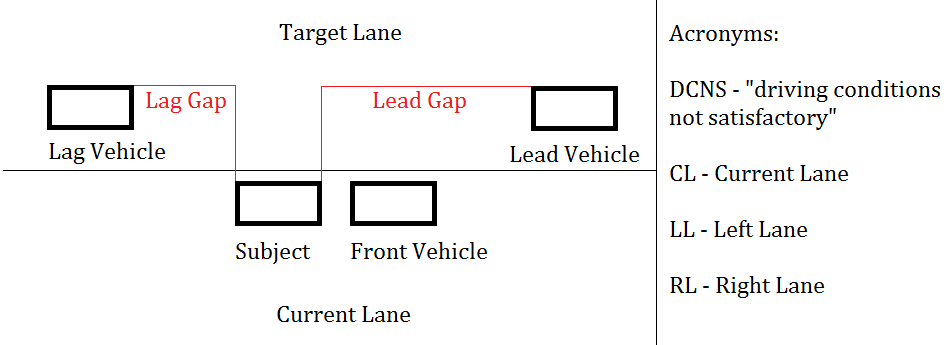
\includegraphics[width=\linewidth]{Lane_Changing_Graphic.png}
  %~ 
\includegraphics[width=\linewidth]{kitty.jpg}
  \caption{A potential lane change}
  \label{fig:kitty1}
\end{figure}

The phenomenon of lane changing by drivers is modeled probabilistically by Ahmed in his thesis. We used that model. See Figure \ref{fig:kitty1} for a diagram that with following the discussion.



Here’s a high-level description of the model (Here, $\nu_n$ is a standard normal variable for each person, to capture uncertainty) :

\begin{enumerate}

\item

A human decides whether or not the driving conditions in their lane are satisfactory (DCNS = “driving conditions not satisfactory”). This is given by a binary logit model.

$P_t(DCNS | \nu_n) = (1 + \exp(-X_n^{DCNS}(t)\beta^{DCNS} - \alpha^{DCNS}\nu_n)) ^ {-1}$

This is the probability that the driver finds the conditions in the current lane to be not satisfactory. That’s when the driver considers a lane change. 


\item

After that, the driver looks for an acceptable gap in the neighbouring lane(s). A gap is called acceptable if the lead gap is acceptable and the lag gap is acceptable. 

The lead and lag gaps are acceptable if they each exceed the ‘critical’ gap.

The critical gap is given by this expression:

$G_n^{cr, g} = \exp(X_n^g(t)\beta^g + \alpha^g\nu_n^g(t) + \epsilon_n^g(t)), \ g \in \{lead,\ lag\}$

Assuming $\epsilon^g_n(t) \sim N(0, \sigma_{\epsilon^g}^2)$, $G^{cr}$s are then log-normally distributed.

$P_t(gap\ acceptable) = P_t(lead\ gap\ acceptable) P_t(lag\ gap\ acceptable)$

 	$ = P(G^{lead}_n(t) > G^{cr, lead}_n(t) | \nu_n) P(G^{lag}_n(t) > G^{cr, lag}_n(t) | \nu_n) $


$ = P(ln(G^{lead}_n(t)) > ln(G^{cr, lead}_n(t)) | \nu_n) P(ln(G^{lag}_n(t)) > ln(G^{cr, lag}_n(t)) | \nu_n) $

$  = \Phi\left(
   \frac{
       \ln(G^{lead}_n(t)) - X_n^{lead}(t)\beta^{lead} - \alpha^{lead}\nu_n
   }{
       \sigma_{\epsilon^{lead}}
   }
\right)
\Phi\left(
   \frac{
       \ln(G^{lag}_n(t)) - X_n^{lag}(t)\beta^{lag} - \alpha^{lag}\nu_n
   }{
       \sigma_{\epsilon^{lag}}
   }
\right)
         $

\item
So then, given DCNS and $\nu_n$, the probability of switching to the left lane is given by:

         $ P_t(Left Lane (LL) | DCNS, \nu_n) = \frac{1}{1 + \exp(-X_n^{LL}\beta^{LL} - \alpha^{LL}\nu_n)} $

\item
To put it all together:	

            $ P_t(LL | \nu_n) = P_t(gap\ acceptable for\ LL) P(LL | DCNS,\ \nu_n) P(DCNS | \nu_n) $

        $P_t(RL | \nu_n)$ can be similarly calculated, and simply, $P(CL | \nu_n) = 1 - (P_t(RL | \nu_n) + P_t(LL | \nu_n))$

\end{enumerate}

The model parameters, including which variables were the most important, and what weights/parameters to use for them, were estimated using data from Interstate 93 in Boston. Here is what we have:

\noindent 

$X_n^{DCNS} =
\begin{bmatrix}
    1 \\ \\
    subject\ speed - desired\ speed  \\ \\
    tailgate \\ \\
\end{bmatrix}
\beta^{DCNS} = \begin{bmatrix}
    0.225\\
    -0.0658\\
    0.423\\
\end{bmatrix}
\alpha^{DCNS} = -1.11\\
$

$
\noindent X_n^{lag} = \begin{bmatrix}
    1 \\ \\
    min(0, lag\ vehicle\ speed - subject\ speed)  \\ \\
    max(0, lag\ vehicle\ speed - subject\ speed)  \\ \\
\end{bmatrix}
\beta^{lag} = \begin{bmatrix}
    2.02\\
    0.153\\
    0.188\\
\end{bmatrix}
\begin{bmatrix}
    \alpha^{lag} \\
    \ln(\sigma_{\epsilon^{lag}})\\
\end{bmatrix} = \begin{bmatrix}
    -0.653 \\
    -0.642 \\
\end{bmatrix}\\
$

$\noindent X_n^{lead} = \begin{bmatrix}
    1 \\ \\
    min(0, lead\ vehicle\ speed - subject\ speed)  \\ \\
\end{bmatrix}
\beta^{lag} = \begin{bmatrix}
    0.508\\
     -0.420\\
\end{bmatrix}
\begin{bmatrix}
    \alpha^{lead} \\
    \ln(\sigma_{\epsilon^{lead}})\\
\end{bmatrix} = \begin{bmatrix}
    0.727 \\
    -0.717 \\
\end{bmatrix}
$

$\noindent X_n^{LL} = \begin{bmatrix}
    1 \\ \\
    Lead\ vehicle\ speed - desired\ speed  \\ \\
    Front\ vehicle\ speed - desired\ speed  \\ \\
    Lag\ vehicle\ speed - subject\ speed  \\ \\
\end{bmatrix}
$
$
\beta^{LL} = \begin{bmatrix}
    -1.87\\
    0.0328\\
    -0.158\\
    -0.0960\\
\end{bmatrix}
    \alpha^{LL} = -0.246 
$

\chapter{Autonomous Car Driving}
\thispagestyle{fancy} % this is magic. put it after every \chapter{...}
\section{Optimal Car Following Strategies}

Kitties are fluffy and make great space fillers.

\section{Optimal Lane Changing Strategies}
I’m rubber. You’re glue.

\section{Hive Mind Optimizations}
Glue can’t speak. You try to scream but your mouth fills with glue.

\chapter{Applying the Simulator}
\thispagestyle{fancy} % this is magic. put it after every \chapter{...}
\section{Preparing the data}
I wrap my rubber arms around your sticky bulk. Your neoprene base bonds instantly with my surface.
\section{Running simulations}
You’re glue. I’m rubber. Staring at you with my dead rubber eyes. Forever.

%%% Local Variables:
%%% mode: latex
%%% TeX-master: "main"
%%% End:

\begin{thebibliography}{9}

\bibitem{jiang}
	Tao Jiang, Srdjan Petrovic, Uma Ayyer, Anand Tolani, Sajid Husain
	Self-Driving Cars: Disruptive or Incremental?,
	Applied Innovation Review,
	Issue 1,
	June 2015.
	%http://cet.berkeley.edu/wp-content/uploads/Self-Driving-Cars.pdf

\bibitem{holland}
	E.N. Holland,
	A generalised stability criterion for motorway traffic,
	ScienceDirect,
	Volume 32,
	Issue 2
	February 1998.
	%http://cet.berkeley.edu/wp-content/uploads/Self-Driving-Cars.pdf

\bibitem{mit}
	Massachusetts Institute of Technology. 
	Mathematicians Take Aim At 'Phantom' Traffic Jams: New Model Could Help Design Better Roads.
	ScienceDaily. 
	ScienceDaily,
	14 June 2009.
	%www.sciencedaily.com/releases/2009/06/090608151550.htm

\bibitem{kerner}
	Boris S. Kerner,
	Introduction to Modern Traffic Flow Theory and Control,
	Springer,
	2009.
	%http://utdallas.primo.hosted.exlibrisgroup.com/primo_library/libweb/action/display.do;jsessionid=9F6B0DCFE6540AD9A066FCB3BF6E5A62?tabs=detailsTab&ct=display&fn=search&doc=UTD_ALMA51156292480001421&indx=1&recIds=UTD_ALMA51156292480001421&recIdxs=0&elementId=0&renderMode=poppedOut&displayMode=full&frbrVersion=&frbg=&dscnt=0&scp.scps=scope%3A%28UTD_ALMA%29&tb=t&mode=Basic&vid=UTDALMA&srt=rank&tab=catalog&vl(freeText0)=Introduction%20to%20Modern%20Traffic%20Flow%20Theory%20and%20Control&dum=true&dstmp=1484929904273

\bibitem{treiber}
	Martin Treiber, Ansgar Hennecke, and Dirk Helbing.
	Congested Traffic States in Empirical Observations and Microscopic Simulations
	Institute of Theoretical Physics, University of Stuttgart
	2000
	%~ http://journals.aps.org/pre/pdf/10.1103/PhysRevE.62.1805

\bibitem{kesting}
	Arne Kesting, Martin Treiber, and Dirk Helbing.
	Enhanced intelligent Driver Model to Access the Impact of Driving strategies on Traffic Capacity
	Institute for Transport \& Economics
	18 December 2009
	%~ https://arxiv.org/pdf/0912.3613v1.pdf

\bibitem{ahmed}
	Kazi Iftekhar Ahmed
	Modeling Drivers' Acceleration and Lane Changing Behavior
	Massachusetts Institute of Technology 
	1999
	%~ Thesis guy
	%~ https://its.mit.edu/sites/default/files/documents/DRIVIN.PDF

\end{thebibliography}
